% Intended LaTeX compiler: pdflatex
\documentclass[11pt]{article}
\usepackage[utf8]{inputenc}
\usepackage[T1]{fontenc}
\usepackage{graphicx}
\usepackage{longtable}
\usepackage{wrapfig}
\usepackage{rotating}
\usepackage[normalem]{ulem}
\usepackage{amsmath}
\usepackage{amssymb}
\usepackage{capt-of}
\usepackage{hyperref}
\author{Fethi Okyar}
\date{2026-05-11}
\title{Chapter 7: Constitutive Relations\\\medskip
\large Reading: [Fung/94] Chapter 7}
\hypersetup{
 pdfauthor={Fethi Okyar},
 pdftitle={Chapter 7: Constitutive Relations},
 pdfkeywords={},
 pdfsubject={},
 pdfcreator={Emacs 30.2 (Org mode 9.7.11)}, 
 pdflang={English}}
\begin{document}

\maketitle
\setcounter{tocdepth}{1}
\tableofcontents

\section*{(\(\S7.1\)) Definition}
\label{sec:org030592e}
\begin{itemize}
\item Define: the dependent and independent variables of the mechanics of solids and fluid
\item Define: Constitution, constitutional, constitutive
\end{itemize}

\begin{center}
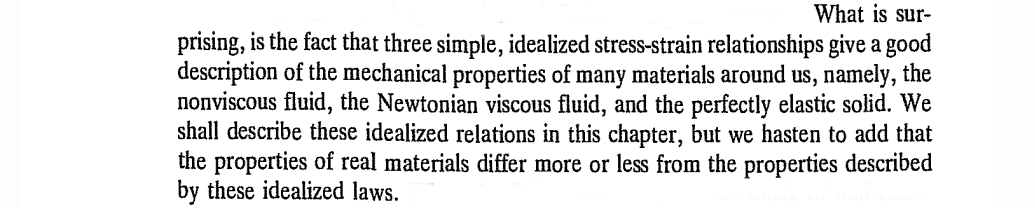
\includegraphics[width=.9\linewidth]{./images/FU94_7.1foreword.png}
\end{center}
\section*{(\(\S7.4\)) Hookean Elastic Solids}
\label{sec:orgfd77701}
\subsection*{Example: Tensile Test}
\label{sec:org598c89b}
\begin{itemize}
\item How do materials respond to strain? or stress??
\end{itemize}
\begin{center}
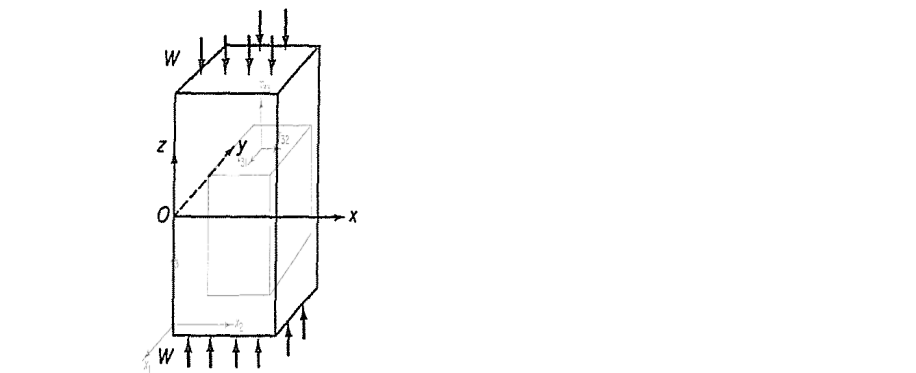
\includegraphics[width=.9\linewidth]{./images/FU94_1.11figure9a-uniaxial.png}
\end{center}

\begin{itemize}
\item \(\epsilon_{33} \to \epsilon\), the normal strain. \(\tau_{33} \to \sigma\), the normal stress.
$$ \epsilon = \kappa \sigma, \hspace{2em} \sigma = E \epsilon $$
\item What is the \emph{modulus of elasticity}, \(E\), of the bar?
\end{itemize}
\subsection*{Generalization}
\label{sec:org8b67cc2}
\begin{itemize}
\item $$ \begin{bmatrix} \tau_{11} & \tau_{12} & \tau_{13} \\ \tau_{21} & \tau_{22} & \tau_{23} \\ \tau_{31} & \tau_{32} & \tau_{33} \end{bmatrix} \hspace{2em} ?? \hspace{2em} \begin{bmatrix} \epsilon_{11} & \epsilon_{12} & \epsilon_{13} \\ \epsilon_{21} & \epsilon_{22} & \epsilon_{23} \\ \epsilon_{31} & \epsilon_{32} & \epsilon_{33} \end{bmatrix} $$
\end{itemize}
\begin{itemize}
\item Connections between the stress and strain components? How many of them are there? \(C_{ijkl}\) ??
\item Write out one component, e.g.,
$$ \tau_{23} = C_{2311} \epsilon_{11} + C_{2312} \epsilon_{12} + C_{2313} \epsilon_{13} \ldots + C_{2333} \epsilon_{33} $$
\item There are eight other such components! \(9\times 9 = 81\) components in \(C_{ijkl}\) !!
\item The general linear stress-strain relation is enclosed within a single indicial expression
$$ \tau_{ij} = C_{ijkl} \epsilon_{kl} $$
\end{itemize}
\subsection*{Reduction}
\label{sec:orgce86193}
\begin{itemize}
\item The actual number of independent material parameters? 81? certainly not!
\item \textbf{Important Note:} Stress is a symmetric tensor! Since \(\tau_{ij} = \tau_{ji}\), we need
$$ C_{ijkl} \epsilon_{kl} = C_{jikl} \epsilon_{kl} \; \forall \, k,l $$
\item This requires that \(C_{ijkl} = C_{jikl}\), and is known as the first \textbf{minor symmetry} in the \(C\) tensor, reducing the number of coefficients, \(81 \to 54\).
\item \textbf{Another Note:} Strain is also symmetric!! By the freedom to arbitrarily assign dummy indices, we get
$$ C_{ijkl} \epsilon_{kl} = C_{ijkl} \epsilon_{lk} = C_{ijlk} \epsilon_{kl} $$
\item This means that \(C_{ijkl} = C_{ijlk}\), and is known as the \textbf{second minor} symmetry, further reducing the number of coefficients, \(54 \to 36\)
\item \textbf{Finally}, it can be shown that the coefficient tensor possesses \textbf{major symmetry} in the dual index pairs.
$$ C_{ijkl} = C_{klij} $$
\item Thus the most general elasticity tensor can be constructed in terms of a total of 21 elastic coefficients.
\end{itemize}
\subsection*{The Voight Solid}
\label{sec:org5db0f23}
\begin{itemize}
\item We reshape the three-by-three stress and strain tensors as one-by-six first order arrays.
$$ \left\{ \begin{array}{c} \tau_{11} \\ \tau_{22} \\ \tau_{33} \\ \tau_{23} \\ \tau_{31} \\ \tau_{12} \end{array} \right\} = \begin{bmatrix} C_{1111} & C_{1122} & C_{1133} & C_{1123} & C_{1113} & C_{1112} \\
    & C_{2222} & C_{2233} & C_{2223} & C_{2213} & C_{2212} \\
    &  & C_{3333} & C_{3323} & C_{3313} & C_{3312} \\
    &  &  & C_{2323} & C_{2313} & C_{2312} \\
    &  \text{sym} &  &  & C_{1313} & C_{1312} \\
    &  &  &  &  & C_{1212}  \end{bmatrix}   \left\{ \begin{array}{c} \epsilon_{11} \\ \epsilon_{22} \\ \epsilon_{33} \\ \epsilon_{23} \\ \epsilon_{31} \\ \epsilon_{12} \end{array} \right\} $$
\end{itemize}
\subsection*{Isotropy}
\label{sec:org24ddffc}
\begin{itemize}
\item Does material behavior change as a function of the stress traction vector?
\item Are material properties a function of the orientation?
\item If the answer is \textbf{no} or \textbf{almost no}, we call the material to be \emph{isotropic}.
\item In this case, the number of independent elasticity coefficients goes down, \(21 \to 2\).
\item For an isotropic material, exactly \emph{two} independent elastic constants are required to characterize the material
\item The constitutive relation for a Hookean solid is called the \emph{Hooke's law} reading
$$ \sigma_{ij} = \lambda \epsilon_{kk} \delta_{ij} + 2 \mu \epsilon_{ij} $$
where \(\lambda\) and \(\mu\) are called \emph{Lame's constants}.
\end{itemize}
\subsubsection*{in extenso}
\label{sec:org04c4e53}
\begin{itemize}
\item It will be useful to expand the Hooke's law from indicial notation to an extensive form
\begin{align}
\sigma_{xx} & = \lambda (\epsilon_{xx} + \epsilon_{yy} + \epsilon_{zz}) + 2 G \epsilon_{xx} \\
\sigma_{yy} & = \lambda (\epsilon_{xx} + \epsilon_{yy} + \epsilon_{zz}) + 2 G \epsilon_{yy} \\
\sigma_{zz} & = \lambda (\epsilon_{xx} + \epsilon_{yy} + \epsilon_{zz}) + 2 G \epsilon_{zz} \end{align}
$$ \sigma_{yz} = G \epsilon_{yz}, \hspace{2em} \sigma_{zx} = G \epsilon_{zx}, \hspace{2em} \sigma_{xy} = G \epsilon_{xy} $$
where \(G=\mu\) is a constant known as the \emph{shear modulus}.
\end{itemize}
\subsubsection*{Inversion}
\label{sec:orgad795d6}
\begin{itemize}
\item These equations can be inverted to write the strains in terms of stresses.
\item It is customary to introduce \textbf{another pair} of material parameters in writing the inverted form of constitutive relations: the elastic modulus, \(E\), and the Poisson's ratio, \(\nu\). These are related with \(\lambda\) and \(\mu\).
\item The inverted form reads
\begin{center}
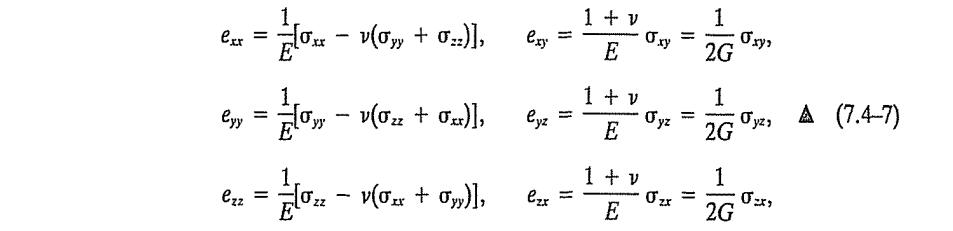
\includegraphics[width=.9\linewidth]{./images/FU94_7.4equation7.png}
\end{center}
\end{itemize}
\section*{Fluids}
\label{sec:org30626aa}
\begin{itemize}
\item The independent variable describing a fluid motion is the \emph{velocity}.
\end{itemize}
\begin{itemize}
\item 
\end{itemize}
\end{document}
